%! Licence = CC BY-NC-SA 4.0

%! Author = gianfluetsch, mariuszindel
%! Date = 19. Jan 2022
%! Project = pfsec_summary

\section{Platform Security}
Platform Security bezieht sich auf die Sicherheitsarchitektur, Werkzeuge und Prozesse, die die Sicherheit einer gesamten Computerplattform gewährleisten. Sie verwendet gebündelte/vereinheitlichte Sicherheitssoftware, Systeme und Prozesse, um die Sicherheit der Hardware, der Software, des Netzes, des Speichers und anderer Komponenten einer Computerplattform zu gewährleisten.\\

Die Platform Security ermöglicht die Sicherung einer gesamten Plattform durch eine zentrale Sicherheitsarchitektur oder ein zentrales Sicherheitssystem. Im Gegensatz zu einem mehrschichtigen Sicherheitsansatz, bei dem jede Schicht/jedes System seine eigene Sicherheit verwaltet, sichert die Plattformsicherheit alle Komponenten und Schichten innerhalb einer Plattform. Dies ermöglicht die Eliminierung einzelner Sicherheitsmaßnahmen und die Verwendung mehrerer Anwendungen/Dienste zur Sicherung verschiedener Schichten einer IT-Umgebung.

\subsection{Security Services through security controls}
\begin{center}
    \vspace{-8pt}
    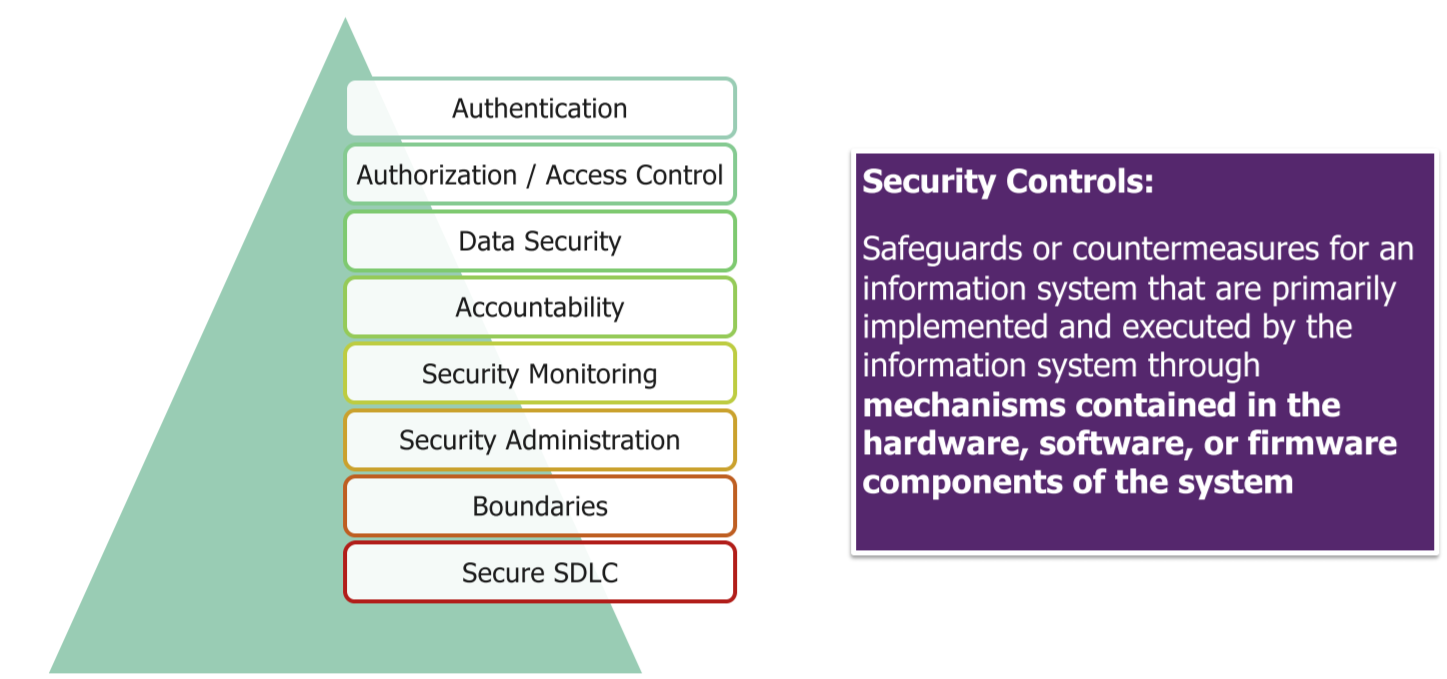
\includegraphics[width=.8\linewidth]{01-platform_security/security_services}
    \vspace{-8pt}
\end{center}

\subsection{Security Architecture}

\subsubsection{Characteristics}
\begin{itemize}
    \item Eine Sicherheitsarchitektur ist ein \textbf{einheitlicher} Sicherheitsentwurf, der sich mit den Notwendigkeiten und potenziellen Risiken in einem \textbf{bestimmten Szenario oder einer bestimmten Umgebung} befasst.
    \item Sie legt auch fest, \textbf{wann und wo Sicherheitskontrollen durchgeführt} werden sollen.
    \item In einer Sicherheitsarchitektur werden die \textbf{Entwurfsprinzipien} klar dargelegt, und \textbf{detaillierte Spezifikationen} der Sicherheitskontrollen werden im Allgemeinen in unabhängigen Dokumenten dokumentiert.
    \item Eine Sicherheitsarchitektur kann als ein Entwurf betrachtet werden, der eine \textbf{Struktur} umfasst und die \textbf{Verbindung zwischen den Komponenten} dieser Struktur behandelt
    \item Eine Sicherheitsarchitektur ist ein präskriptives Dokument, das eine \textbf{Reihe von kohärenten Modellen und Prinzipien} verwendet, um die Umsetzung der Informationssicherheitspolitik einer Organisation anzuleiten.
\end{itemize}

\subsubsection{Key Characteristics}
\begin{itemize}
    \item Sie besteht aus einem \textbf{transparenten und kohärenten Überblick über Modelle, Grundsätze, Ausgangspunkte und Bedingungen}, die eine konkrete Auslegung der Informationssicherheitspolitik ermöglichen, ohne dass in der Regel konkrete Lösungen genannt werden. spezifische Lösungen zu sprechen.
    \item Sie \textbf{reduziert ein komplexes Problem} auf Modelle, Prinzipien und Teilprobleme, die es zu verstehen gilt.
    \item Ziel ist eine gute Verständlichkeit zu erreichen, auch wenn das Problem sehr komplex ist
    \item Die Modelle und Grundsätze \textbf{zeigen, wo Sie welche Art von Maßnahmen ergreifen, wann die Grundsätze anwendbar sind und wie sie mit anderen Grundsätzen mit anderen Prinzipien zusammenhängen}.
\end{itemize}

\subsection{Basic Security Design Principles}
\begin{center}
    \vspace{-8pt}
    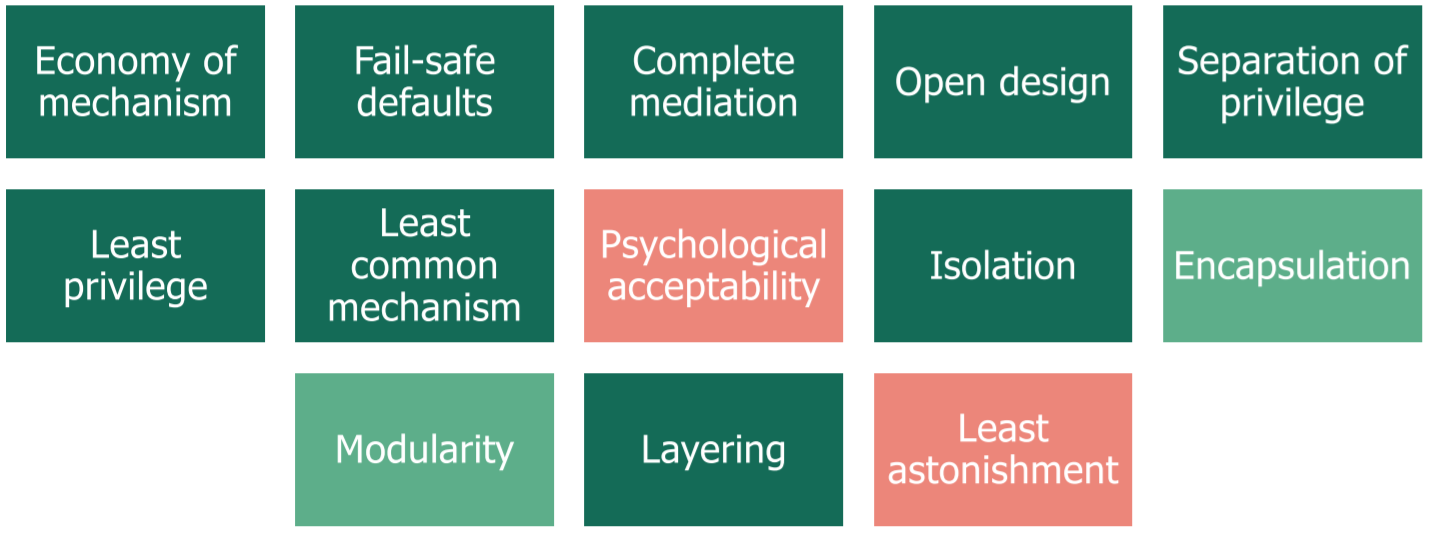
\includegraphics[width=.8\linewidth]{01-platform_security/security_design_principles}
    \vspace{-8pt}
\end{center}

\begin{itemize}
    \item \textbf{Economy of mechanism}:
    \begin{itemize}
        \item KISS
    \end{itemize}
    \item \textbf{Fail-safe defaults}: 
    \begin{itemize}
        \item Access Decision sollte bei Fehler in Safe\-State fallen $\rightarrow$ Was ist erlaubt \& nicht was ist verboten (positiver Ansatz)
    \end{itemize}
    \item \textbf{Complete mediation}: 
    \begin{itemize}
        \item Jeder Access sollte überprüft sein (keine Blindgänger im System)
    \end{itemize}
    \item \textbf{Open design}: 
    \begin{itemize}
        \item Design bietet keine Angriffsfläche auch wenn man es kennt (da es z.B. open-source ist)
    \end{itemize}
    \item \textbf{Separation of privilege}:
    \begin{itemize}
        \item starke Authentifizierung (2FA) bringt nichts, wenn der Admin trotzdemnoch mit username + PW aufs System kommt
    \end{itemize}
    \item \textbf{Least privilege}: 
    \begin{itemize}
        \item nicht alles als root
    \end{itemize}
    \item \textbf{Least common mechanism}: 
    \begin{itemize}
        \item gleicher Mechanismus wird für unterschiedliche Zwecke eingesetzt $\rightarrow$ Gefahr für weakest Link
    \end{itemize}
    \item \textbf{Psychological acceptability}: 
    \begin{itemize}
        \item Was kauft der User ab, das er wirklich machen muss dass ein System sicherer wird (Tempobeschränkung auf Strasse mit Blitzer funktioniert nur beschränkt $\rightarrow$ besser mit Überzeugung arbeiten, wieso Temporeduzierung nötig ist)
    \end{itemize}
    \item \textbf{Isolation}: 
    \begin{itemize}
        \item System soll nicht direkt unter Beschus stehen $\rightarrow$ mehrere isolierte Layer mit FW etc. haben
    \end{itemize}
    \item \textbf{Encapsulation}: 
    \begin{itemize}
        \item eigene Domain
    \end{itemize}
    \item \textbf{Modularity}: 
    \begin{itemize}
        \item Module separieren/ trennen
    \end{itemize}
    \item \textbf{Layering}: 
    \begin{itemize}
        \item defense in depth
    \end{itemize}
    \item \textbf{Least astonishment}: 
    \begin{itemize}
        \item ein Programm/eine Benutzeroberfläche sollte so reagieren, dass der Benutzer möglichst wenig überrascht wird.
    \end{itemize}
\end{itemize}

\subsubsection{Architecting a Secure Digital World}
\begin{center}
    \vspace{-8pt}
    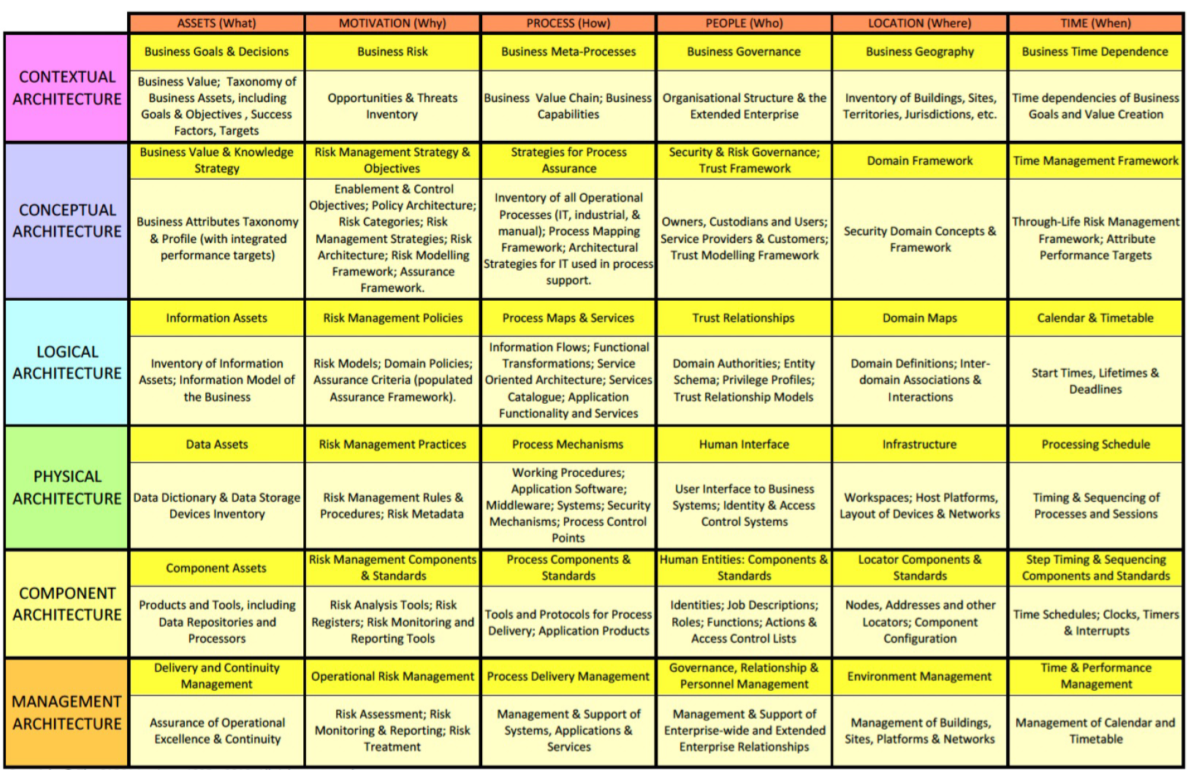
\includegraphics[width=1.0\linewidth]{01-platform_security/secure_digital_world}
    \vspace{-8pt}
\end{center}

\subsection{Examples}

\subsubsection{IAM - Identity and Access Management}
\begin{center}
    \vspace{-8pt}
    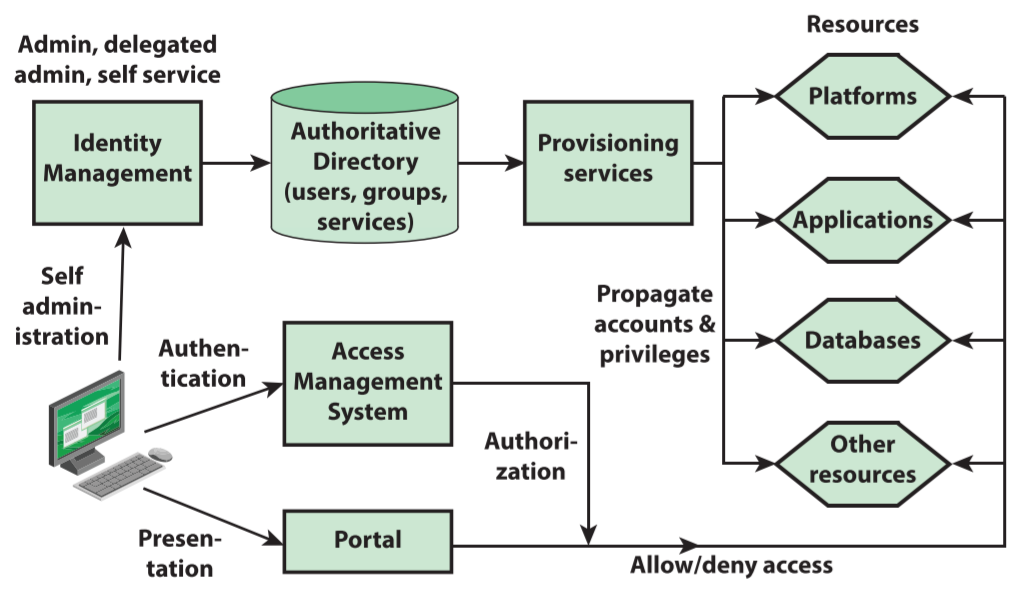
\includegraphics[width=.7\linewidth]{01-platform_security/iam}
    \vspace{-8pt}
\end{center}

\subsubsection{Malware Protection}
\begin{center}
    \vspace{-8pt}
    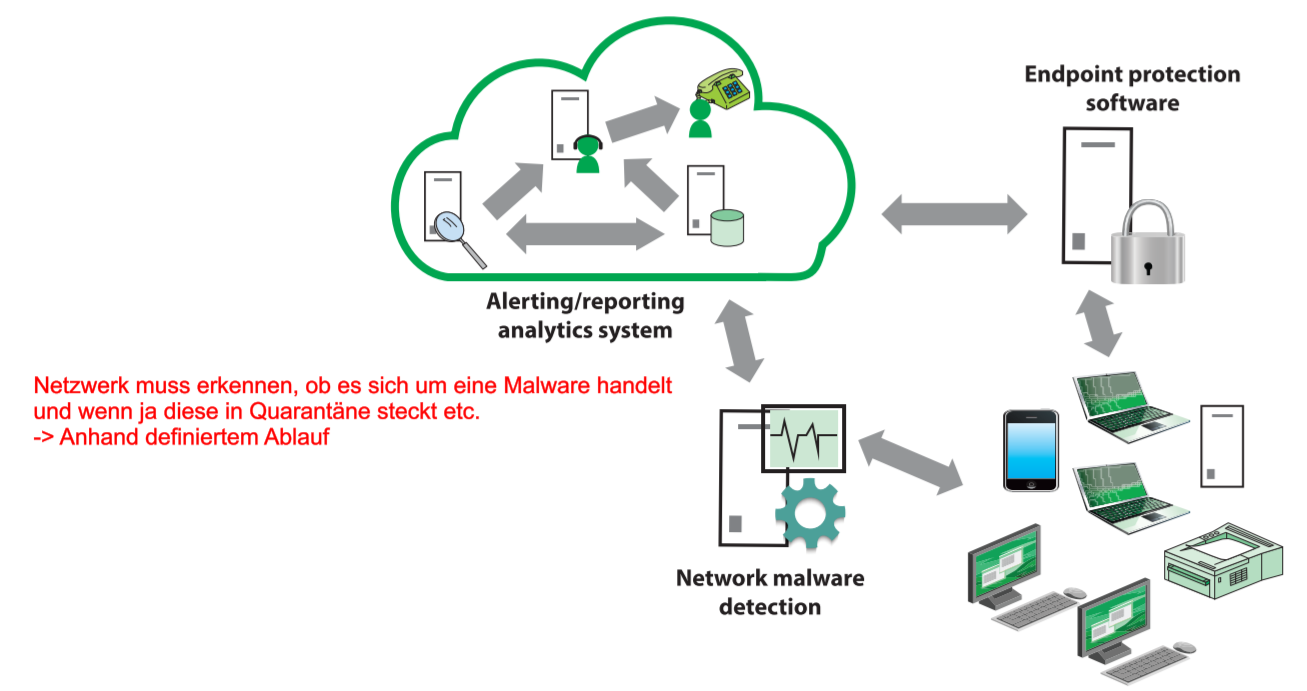
\includegraphics[width=.8\linewidth]{01-platform_security/malware_protection}
    \vspace{-8pt}
\end{center}

\subsubsection{Cryptographic Key Life Cycle}
\begin{center}
    \vspace{-8pt}
    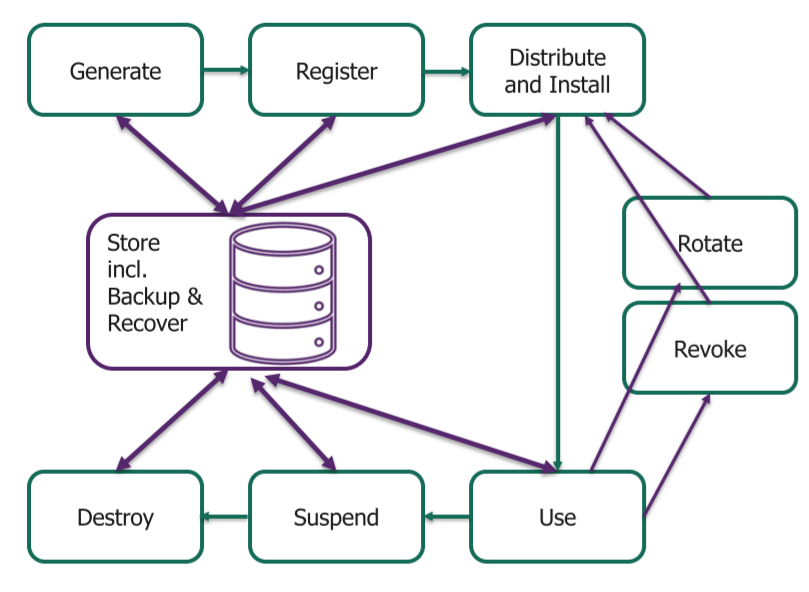
\includegraphics[width=.7\linewidth]{01-platform_security/cryptographic_key_lifecycle}
    \vspace{-8pt}
\end{center}



